\section{DOMÓTICA}

El término domótica proviene de la unión de las palabras \emph{domus} (que significa casa en latín) y \emph{tica} (de automática, palabra en griego). La Real Academia Española lo define como el <<conjunto de sistemas que automatizan las diferentes instalaciones de una vivienda>>.

En este proyecto se utilizará el concepto de domótica como la tecnología aplicada al Internet de las Cosas en el hogar, es decir, conectar nuestro hogar a la nube.

\subsection{Historia}

\parpic[r][]{
    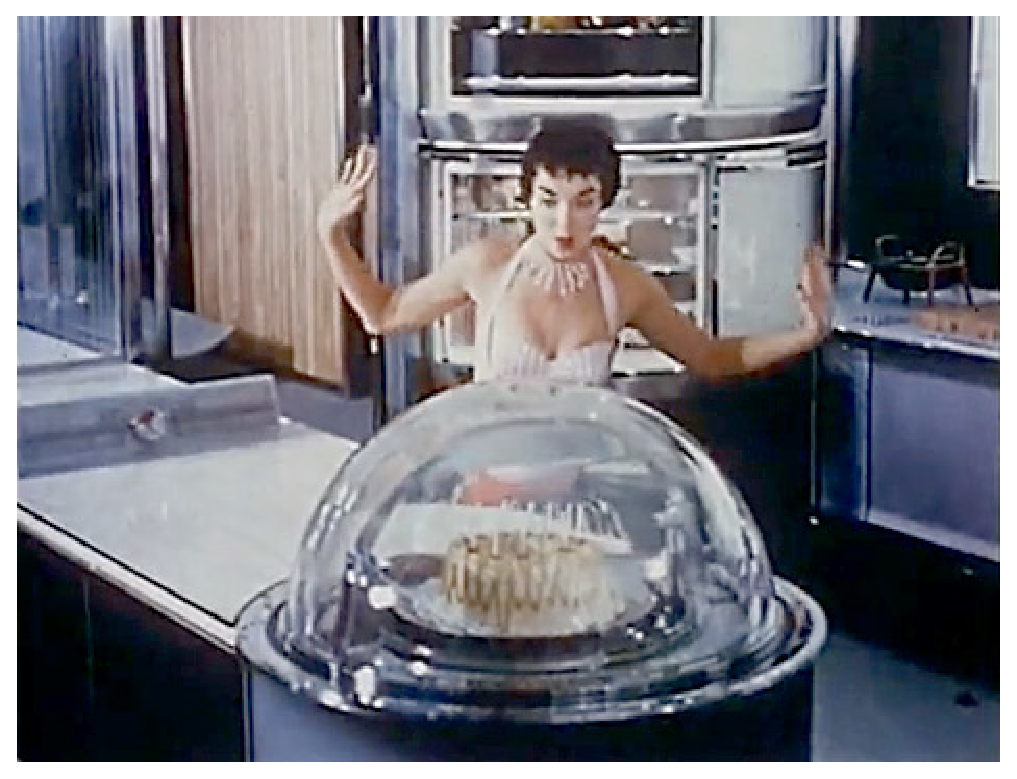
\includegraphics[keepaspectratio,width=0.25\textwidth]{Design_for_Dreaming_-_Cake_Under_Glass.eps}
    \label{fig:design-for-dreaming}
}

El hogar inteligente y automático comenzó a imaginarse en historias de ciencia ficción a inicios del siglo XX. En 1956 se emitió la película \emph{Design for Dreaming}~\ref{fig:design-for-dreaming} donde una mujer cae dormida y tiene una serie de sueños futuristas, incluyendo a \emph{Frigidaire}, la cocina automatizada del futuro. De ahí que no se pueda establecer una fecha concreta donde establecer el inicio de la domótica.

No obstante, si hemos de establecer una fecha de importante tenemos que hablar de 1975 con la aparición de \emph{X10}, un protocolo de comunicación que básicamente permite el control de las luces del hogar, para ello, utiliza la línea eléctrica como medio de comunicación. Debido a las limitaciones del protocolo de comunicación\emph{X10} se han desarrollado nuevas tecnologías para suplir estas carencias; CEBus, EIB, KNX...

A continuación se va a dar una breve explicación de cada una de estas tecnologías existentes en el mercado.

\subsection{X10}

\emph{X10} es un protocolo de comunicación para el control remoto de dispositivos eléctricos. Fue desarrollado en 1978 por \emph{Pico Electronics of Glenrothes}, Escocia, siendo la primera tecnología domótica en aparecer.

\parpic[r][]{
    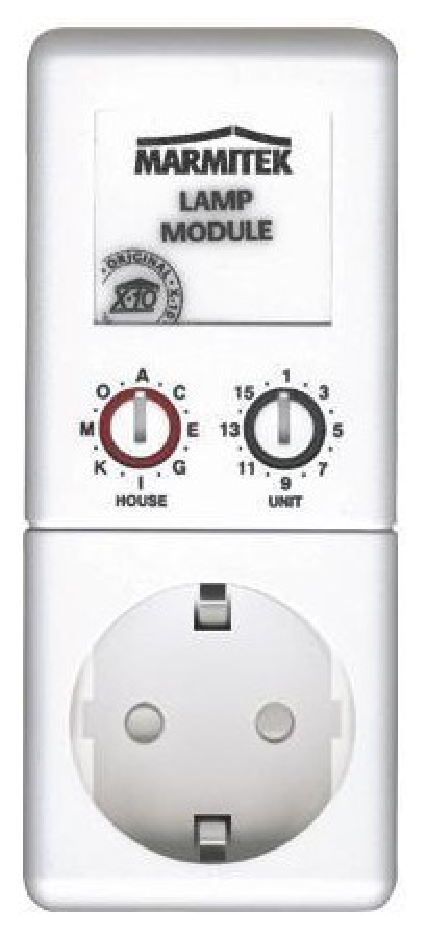
\includegraphics[keepaspectratio,width=0.09\textwidth]{modulo-lampara-x10.eps}
    \label{fig:modulo-lampara-x10}
}

Utiliza el cableado eléctrico como medio de comunicación que, debido a la limitación en ancho de banda que proporciona, solo es capaz de soportar hasta 256 dispositivos. A pesar de ello, es una tecnología ampliamente utilizada en Norteamérica y Europa por su característica de autoinstalable, sin necesidad de cableado adicional.

Las señales de control de X10 se basan en la transmisión de ráfagas de pulsos de \emph{RF} (120 kHz) que representan información digital. Estos pulsos se sincronizan en el cruce por cero de la señal de red (50 Hz ó 60 Hz). Con la presencia de un pulso en un semiciclo y la ausencia del mismo en el semiciclo siguiente se representa un '1' lógico y a la inversa se representa un '0'. A su vez, cada orden se transmite 2 veces, con lo cual toda la información transmitida tiene cuádruple redundancia. Cada orden involucra 11 ciclos de red (220 ms para 50 Hz y 183,33, para 60Hz).

Primero se transmite una orden con el Código de Casa y el Número de Módulo que direccionan el módulo en cuestión. Luego se transmite otro orden con el código de función a realizar (Function Code): Apagar/Encender todas las unidades, apagar/encender una unidad, comprobar el estado de una o varias unidades...

\subsection{CEBus}

Bajo la necesidad de mejorar la limitada capacidad del protocolo \emph{X10} surgió \emph{CEBus}. El estándar \emph{CEBus} se desarrolló por la EIA (Electronic Industries Allianza) y su primera especificación salió en 1992.

\emph{CEBus}, a diferencia de \emph{X10}, se comunica sobre varias tecnologías; cableado eléctrico; cable coaxial; infrarrojos; radio frecuencia y cable óptico. Y además, se prescinde de un controlador central distribuyéndose la inteligencia entre todos los componentes del sistema.

Para la comunicación entre distintos medios físicos se necesita utilizar un router intermedio. La información se transmite en forma de mensajes a través de una dirección broadcast o una específica al dispositivo receptor (cada aparato \emph{CEBus} tiene una dirección única asignada).

Por último, se definió un lenguaje orientado a objetos para el control de los dispositivos \emph{CEBus} llamado \emph{CAL} (Common Appliance Language).

\subsection{EIB}

El European Installation Bus (\emph{EIB}) es un sistema domótico impulsado por la Unión Europea, en concreto, por la \emph{EIBA}, una asociación de empresas líderes en instalaciones eléctricas. El objetivo era crear un estándar europeo, y de esta manera, competir contra la importación de productos norteamericanos y japoneses.

\emph{EIB} utiliza un solo bus de comunicación, reduciendo el tiempo de instalación, aunque a diferencia de \emph{CEBus} es necesaria la instalación de su propio cableado. Permite unir hasta 64 dispositivos bajo una sola línea, y mediante acopladores un total de 256 aparatos. Al igual que \emph{CEBus} no es necesario un puesto de control central ya que el sistema trabaja de forma centralizada comunicándose a través del modelo OSI.

Debido al impulso de la Unión Europea y al tratarse de un estándar existen muchos fabricantes de productos \emph{EIB} siendo compatibles entre ellos. Se ha creado una asociación de más de cien miembros y existiendo unas veinte empresas que suministran productos, siendo las más importantes \emph{Siemens}, \emph{ABB}, \emph{Temper}, \emph{Grasslin} y \emph{Niessen}.

\subsection{KNX}

\emph{KNX} es el sucesor y la convergencia de tres estándares previos: el European Home System Protocol (EHS), BâtiBUS, y el European Installation Bus (\emph{EIB}). En 2002 se publicó la especificación \emph{KNX}, permitiendo competir en calidad, prestaciones y precios con otros sistemas existentes, ya que reúne las mejores características de sus predecesores.


El estándar KNX permite el uso de cuatro medios de comunicación; TP (\emph{Twisted Pais}), PL (\emph{Power Line}), RF (\emph{Radio Frequency}) e IP (\emph{Ethernet}). Al igual que sus predecesores es un sistema descentralizado por lo cual no es necesario la utilización de un controlador principal.